% Generated by ArticleSignalDiagrams. Opaque vector fills only.
\documentclass[10pt,tikz,border=5pt]{standalone}
\usepackage{lmodern}
\usetikzlibrary{fit}
\begin{document}
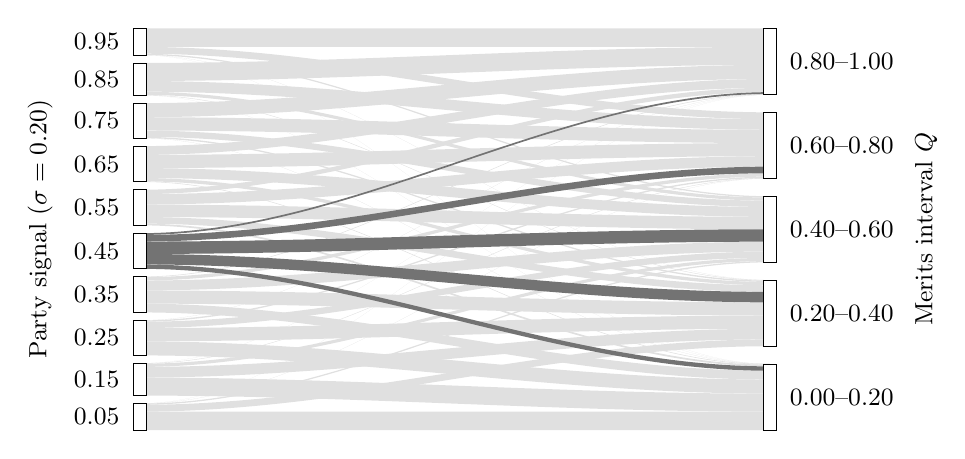
\begin{tikzpicture}[x=1cm,y=1cm,font=\small]\path[fill=black!12,draw=none] (3.3,-5.1) .. controls (6,-5.1) and (8.6,-5.1) .. (11.3,-5.1) -- (11.3,-4.866395) .. controls (8.6,-4.866395) and (6,-4.866395) .. (3.3,-4.866395) -- cycle;
\path[fill=black!12,draw=none] (3.3,-4.866395) .. controls (6,-4.866395) and (8.6,-4.035) .. (11.3,-4.035) -- (11.3,-3.948562) .. controls (8.6,-3.948562) and (6,-4.779957) .. (3.3,-4.779957) -- cycle;
\path[fill=black!12,draw=none] (3.3,-4.779957) .. controls (6,-4.779957) and (8.6,-2.97) .. (11.3,-2.97) -- (11.3,-2.953604) .. controls (8.6,-2.953604) and (6,-4.763561) .. (3.3,-4.763561) -- cycle;
\path[fill=black!12,draw=none] (3.3,-4.763561) .. controls (6,-4.763561) and (8.6,-1.905) .. (11.3,-1.905) -- (11.3,-1.903614) .. controls (8.6,-1.903614) and (6,-4.762175) .. (3.3,-4.762175) -- cycle;
\path[fill=black!12,draw=none] (3.3,-4.762175) .. controls (6,-4.762175) and (8.6,-0.84) .. (11.3,-0.84) -- (11.3,-0.839945) .. controls (8.6,-0.839945) and (6,-4.762119) .. (3.3,-4.762119) -- cycle;
\path[fill=black!12,draw=none] (3.3,-4.662119) .. controls (6,-4.662119) and (8.6,-4.866395) .. (11.3,-4.866395) -- (11.3,-4.637558) .. controls (8.6,-4.637558) and (6,-4.433281) .. (3.3,-4.433281) -- cycle;
\path[fill=black!12,draw=none] (3.3,-4.433281) .. controls (6,-4.433281) and (8.6,-3.948562) .. (11.3,-3.948562) -- (11.3,-3.813554) .. controls (8.6,-3.813554) and (6,-4.298273) .. (3.3,-4.298273) -- cycle;
\path[fill=black!12,draw=none] (3.3,-4.298273) .. controls (6,-4.298273) and (8.6,-2.953604) .. (11.3,-2.953604) -- (11.3,-2.913018) .. controls (8.6,-2.913018) and (6,-4.257687) .. (3.3,-4.257687) -- cycle;
\path[fill=black!12,draw=none] (3.3,-4.257687) .. controls (6,-4.257687) and (8.6,-1.903614) .. (11.3,-1.903614) -- (11.3,-1.898156) .. controls (8.6,-1.898156) and (6,-4.252229) .. (3.3,-4.252229) -- cycle;
\path[fill=black!12,draw=none] (3.3,-4.252229) .. controls (6,-4.252229) and (8.6,-0.839945) .. (11.3,-0.839945) -- (11.3,-0.839594) .. controls (8.6,-0.839594) and (6,-4.251878) .. (3.3,-4.251878) -- cycle;
\path[fill=black!12,draw=none] (3.3,-4.151878) .. controls (6,-4.151878) and (8.6,-4.637558) .. (11.3,-4.637558) -- (11.3,-4.458606) .. controls (8.6,-4.458606) and (6,-3.972926) .. (3.3,-3.972926) -- cycle;
\path[fill=black!12,draw=none] (3.3,-3.972926) .. controls (6,-3.972926) and (8.6,-3.813554) .. (11.3,-3.813554) -- (11.3,-3.645357) .. controls (8.6,-3.645357) and (6,-3.80473) .. (3.3,-3.80473) -- cycle;
\path[fill=black!12,draw=none] (3.3,-3.80473) .. controls (6,-3.80473) and (8.6,-2.913018) .. (11.3,-2.913018) -- (11.3,-2.833036) .. controls (8.6,-2.833036) and (6,-3.724749) .. (3.3,-3.724749) -- cycle;
\path[fill=black!12,draw=none] (3.3,-3.724749) .. controls (6,-3.724749) and (8.6,-1.898156) .. (11.3,-1.898156) -- (11.3,-1.88109) .. controls (8.6,-1.88109) and (6,-3.707683) .. (3.3,-3.707683) -- cycle;
\path[fill=black!12,draw=none] (3.3,-3.707683) .. controls (6,-3.707683) and (8.6,-0.839594) .. (11.3,-0.839594) -- (11.3,-0.837838) .. controls (8.6,-0.837838) and (6,-3.705927) .. (3.3,-3.705927) -- cycle;
\path[fill=black!12,draw=none] (3.3,-3.605927) .. controls (6,-3.605927) and (8.6,-4.458606) .. (11.3,-4.458606) -- (11.3,-4.346892) .. controls (8.6,-4.346892) and (6,-3.494213) .. (3.3,-3.494213) -- cycle;
\path[fill=black!12,draw=none] (3.3,-3.494213) .. controls (6,-3.494213) and (8.6,-3.645357) .. (11.3,-3.645357) -- (11.3,-3.478121) .. controls (8.6,-3.478121) and (6,-3.326977) .. (3.3,-3.326977) -- cycle;
\path[fill=black!12,draw=none] (3.3,-3.326977) .. controls (6,-3.326977) and (8.6,-2.833036) .. (11.3,-2.833036) -- (11.3,-2.70741) .. controls (8.6,-2.70741) and (6,-3.201351) .. (3.3,-3.201351) -- cycle;
\path[fill=black!12,draw=none] (3.3,-3.201351) .. controls (6,-3.201351) and (8.6,-1.88109) .. (11.3,-1.88109) -- (11.3,-1.838652) .. controls (8.6,-1.838652) and (6,-3.158913) .. (3.3,-3.158913) -- cycle;
\path[fill=black!12,draw=none] (3.3,-3.158913) .. controls (6,-3.158913) and (8.6,-0.837838) .. (11.3,-0.837838) -- (11.3,-0.830851) .. controls (8.6,-0.830851) and (6,-3.151926) .. (3.3,-3.151926) -- cycle;
\path[fill=black!12,draw=none] (3.3,-2.5) .. controls (6,-2.5) and (8.6,-4.291246) .. (11.3,-4.291246) -- (11.3,-4.269149) .. controls (8.6,-4.269149) and (6,-2.477903) .. (3.3,-2.477903) -- cycle;
\path[fill=black!12,draw=none] (3.3,-2.477903) .. controls (6,-2.477903) and (8.6,-3.345397) .. (11.3,-3.345397) -- (11.3,-3.261348) .. controls (8.6,-3.261348) and (6,-2.393854) .. (3.3,-2.393854) -- cycle;
\path[fill=black!12,draw=none] (3.3,-2.393854) .. controls (6,-2.393854) and (8.6,-2.55) .. (11.3,-2.55) -- (11.3,-2.39259) .. controls (8.6,-2.39259) and (6,-2.236444) .. (3.3,-2.236444) -- cycle;
\path[fill=black!12,draw=none] (3.3,-2.236444) .. controls (6,-2.236444) and (8.6,-1.754603) .. (11.3,-1.754603) -- (11.3,-1.621879) .. controls (8.6,-1.621879) and (6,-2.10372) .. (3.3,-2.10372) -- cycle;
\path[fill=black!12,draw=none] (3.3,-2.10372) .. controls (6,-2.10372) and (8.6,-0.808754) .. (11.3,-0.808754) -- (11.3,-0.753108) .. controls (8.6,-0.753108) and (6,-2.048074) .. (3.3,-2.048074) -- cycle;
\path[fill=black!12,draw=none] (3.3,-1.948074) .. controls (6,-1.948074) and (8.6,-4.269149) .. (11.3,-4.269149) -- (11.3,-4.262162) .. controls (8.6,-4.262162) and (6,-1.941087) .. (3.3,-1.941087) -- cycle;
\path[fill=black!12,draw=none] (3.3,-1.941087) .. controls (6,-1.941087) and (8.6,-3.261348) .. (11.3,-3.261348) -- (11.3,-3.21891) .. controls (8.6,-3.21891) and (6,-1.898649) .. (3.3,-1.898649) -- cycle;
\path[fill=black!12,draw=none] (3.3,-1.898649) .. controls (6,-1.898649) and (8.6,-2.39259) .. (11.3,-2.39259) -- (11.3,-2.266964) .. controls (8.6,-2.266964) and (6,-1.773023) .. (3.3,-1.773023) -- cycle;
\path[fill=black!12,draw=none] (3.3,-1.773023) .. controls (6,-1.773023) and (8.6,-1.621879) .. (11.3,-1.621879) -- (11.3,-1.454643) .. controls (8.6,-1.454643) and (6,-1.605787) .. (3.3,-1.605787) -- cycle;
\path[fill=black!12,draw=none] (3.3,-1.605787) .. controls (6,-1.605787) and (8.6,-0.753108) .. (11.3,-0.753108) -- (11.3,-0.641394) .. controls (8.6,-0.641394) and (6,-1.494073) .. (3.3,-1.494073) -- cycle;
\path[fill=black!12,draw=none] (3.3,-1.394073) .. controls (6,-1.394073) and (8.6,-4.262162) .. (11.3,-4.262162) -- (11.3,-4.260406) .. controls (8.6,-4.260406) and (6,-1.392317) .. (3.3,-1.392317) -- cycle;
\path[fill=black!12,draw=none] (3.3,-1.392317) .. controls (6,-1.392317) and (8.6,-3.21891) .. (11.3,-3.21891) -- (11.3,-3.201844) .. controls (8.6,-3.201844) and (6,-1.375251) .. (3.3,-1.375251) -- cycle;
\path[fill=black!12,draw=none] (3.3,-1.375251) .. controls (6,-1.375251) and (8.6,-2.266964) .. (11.3,-2.266964) -- (11.3,-2.186982) .. controls (8.6,-2.186982) and (6,-1.29527) .. (3.3,-1.29527) -- cycle;
\path[fill=black!12,draw=none] (3.3,-1.29527) .. controls (6,-1.29527) and (8.6,-1.454643) .. (11.3,-1.454643) -- (11.3,-1.286446) .. controls (8.6,-1.286446) and (6,-1.127074) .. (3.3,-1.127074) -- cycle;
\path[fill=black!12,draw=none] (3.3,-1.127074) .. controls (6,-1.127074) and (8.6,-0.641394) .. (11.3,-0.641394) -- (11.3,-0.462442) .. controls (8.6,-0.462442) and (6,-0.948122) .. (3.3,-0.948122) -- cycle;
\path[fill=black!12,draw=none] (3.3,-0.848122) .. controls (6,-0.848122) and (8.6,-4.260406) .. (11.3,-4.260406) -- (11.3,-4.260055) .. controls (8.6,-4.260055) and (6,-0.847771) .. (3.3,-0.847771) -- cycle;
\path[fill=black!12,draw=none] (3.3,-0.847771) .. controls (6,-0.847771) and (8.6,-3.201844) .. (11.3,-3.201844) -- (11.3,-3.196386) .. controls (8.6,-3.196386) and (6,-0.842313) .. (3.3,-0.842313) -- cycle;
\path[fill=black!12,draw=none] (3.3,-0.842313) .. controls (6,-0.842313) and (8.6,-2.186982) .. (11.3,-2.186982) -- (11.3,-2.146396) .. controls (8.6,-2.146396) and (6,-0.801727) .. (3.3,-0.801727) -- cycle;
\path[fill=black!12,draw=none] (3.3,-0.801727) .. controls (6,-0.801727) and (8.6,-1.286446) .. (11.3,-1.286446) -- (11.3,-1.151438) .. controls (8.6,-1.151438) and (6,-0.666719) .. (3.3,-0.666719) -- cycle;
\path[fill=black!12,draw=none] (3.3,-0.666719) .. controls (6,-0.666719) and (8.6,-0.462442) .. (11.3,-0.462442) -- (11.3,-0.233605) .. controls (8.6,-0.233605) and (6,-0.437881) .. (3.3,-0.437881) -- cycle;
\path[fill=black!12,draw=none] (3.3,-0.337881) .. controls (6,-0.337881) and (8.6,-4.260055) .. (11.3,-4.260055) -- (11.3,-4.26) .. controls (8.6,-4.26) and (6,-0.337825) .. (3.3,-0.337825) -- cycle;
\path[fill=black!12,draw=none] (3.3,-0.337825) .. controls (6,-0.337825) and (8.6,-3.196386) .. (11.3,-3.196386) -- (11.3,-3.195) .. controls (8.6,-3.195) and (6,-0.336439) .. (3.3,-0.336439) -- cycle;
\path[fill=black!12,draw=none] (3.3,-0.336439) .. controls (6,-0.336439) and (8.6,-2.146396) .. (11.3,-2.146396) -- (11.3,-2.13) .. controls (8.6,-2.13) and (6,-0.320043) .. (3.3,-0.320043) -- cycle;
\path[fill=black!12,draw=none] (3.3,-0.320043) .. controls (6,-0.320043) and (8.6,-1.151438) .. (11.3,-1.151438) -- (11.3,-1.065) .. controls (8.6,-1.065) and (6,-0.233605) .. (3.3,-0.233605) -- cycle;
\path[fill=black!12,draw=none] (3.3,-0.233605) .. controls (6,-0.233605) and (8.6,-0.233605) .. (11.3,-0.233605) -- (11.3,-0) .. controls (8.6,-0) and (6,0) .. (3.3,0) -- cycle;
\path[fill=black!55,draw=none] (3.3,-3.051926) .. controls (6,-3.051926) and (8.6,-4.346892) .. (11.3,-4.346892) -- (11.3,-4.291246) .. controls (8.6,-4.291246) and (6,-2.99628) .. (3.3,-2.99628) -- cycle;
\path[fill=black!55,draw=none] (3.3,-2.99628) .. controls (6,-2.99628) and (8.6,-3.478121) .. (11.3,-3.478121) -- (11.3,-3.345397) .. controls (8.6,-3.345397) and (6,-2.863556) .. (3.3,-2.863556) -- cycle;
\path[fill=black!55,draw=none] (3.3,-2.863556) .. controls (6,-2.863556) and (8.6,-2.70741) .. (11.3,-2.70741) -- (11.3,-2.55) .. controls (8.6,-2.55) and (6,-2.706146) .. (3.3,-2.706146) -- cycle;
\path[fill=black!55,draw=none] (3.3,-2.706146) .. controls (6,-2.706146) and (8.6,-1.838652) .. (11.3,-1.838652) -- (11.3,-1.754603) .. controls (8.6,-1.754603) and (6,-2.622097) .. (3.3,-2.622097) -- cycle;
\path[fill=black!55,draw=none] (3.3,-2.622097) .. controls (6,-2.622097) and (8.6,-0.830851) .. (11.3,-0.830851) -- (11.3,-0.808754) .. controls (8.6,-0.808754) and (6,-2.6) .. (3.3,-2.6) -- cycle;
\coordinate (axis-midline-0) at (0,-2.55);
\path[fill=white,draw=black,line width=0.3pt] (3.22,-5.1) rectangle (3.38,-4.762119);
\node[anchor=east,fill=white,inner sep=2pt] (bucket-0-0-0) at (3.12,-4.93106) {0.05};
\path[fill=white,draw=black,line width=0.3pt] (3.22,-4.662119) rectangle (3.38,-4.251878);
\node[anchor=east,fill=white,inner sep=2pt] (bucket-0-0-1) at (3.12,-4.456999) {0.15};
\path[fill=white,draw=black,line width=0.3pt] (3.22,-4.151878) rectangle (3.38,-3.705927);
\node[anchor=east,fill=white,inner sep=2pt] (bucket-0-0-2) at (3.12,-3.928902) {0.25};
\path[fill=white,draw=black,line width=0.3pt] (3.22,-3.605927) rectangle (3.38,-3.151926);
\node[anchor=east,fill=white,inner sep=2pt] (bucket-0-0-3) at (3.12,-3.378926) {0.35};
\path[fill=white,draw=black,line width=0.3pt] (3.22,-3.051926) rectangle (3.38,-2.6);
\node[anchor=east,fill=white,inner sep=2pt] (bucket-0-0-4) at (3.12,-2.825963) {0.45};
\path[fill=white,draw=black,line width=0.3pt] (3.22,-2.5) rectangle (3.38,-2.048074);
\node[anchor=east,fill=white,inner sep=2pt] (bucket-0-0-5) at (3.12,-2.274037) {0.55};
\path[fill=white,draw=black,line width=0.3pt] (3.22,-1.948074) rectangle (3.38,-1.494073);
\node[anchor=east,fill=white,inner sep=2pt] (bucket-0-0-6) at (3.12,-1.721074) {0.65};
\path[fill=white,draw=black,line width=0.3pt] (3.22,-1.394073) rectangle (3.38,-0.948122);
\node[anchor=east,fill=white,inner sep=2pt] (bucket-0-0-7) at (3.12,-1.171098) {0.75};
\path[fill=white,draw=black,line width=0.3pt] (3.22,-0.848122) rectangle (3.38,-0.437881);
\node[anchor=east,fill=white,inner sep=2pt] (bucket-0-0-8) at (3.12,-0.643001) {0.85};
\path[fill=white,draw=black,line width=0.3pt] (3.22,-0.337881) rectangle (3.38,0);
\node[anchor=east,fill=white,inner sep=2pt] (bucket-0-0-9) at (3.12,-0.16894) {0.95};
\node[fit=(bucket-0-0-0) (bucket-0-0-1) (bucket-0-0-2) (bucket-0-0-3) (bucket-0-0-4) (bucket-0-0-5) (bucket-0-0-6) (bucket-0-0-7) (bucket-0-0-8) (bucket-0-0-9),inner sep=0pt] (source-labels-0) {};
\coordinate (axis-title-0-0) at (source-labels-0.west |- axis-midline-0);
\node[rotate=90,anchor=south,inner sep=0pt] at ([xshift=-0.18cm]axis-title-0-0) {Party signal ($\sigma=0.20$)};
\path[fill=white,draw=black,line width=0.3pt] (11.22,-5.1) rectangle (11.38,-4.26);
\node[anchor=west,fill=white,inner sep=2pt] (bucket-0-1-0) at (11.48,-4.68) {0.00--0.20};
\path[fill=white,draw=black,line width=0.3pt] (11.22,-4.035) rectangle (11.38,-3.195);
\node[anchor=west,fill=white,inner sep=2pt] (bucket-0-1-1) at (11.48,-3.615) {0.20--0.40};
\path[fill=white,draw=black,line width=0.3pt] (11.22,-2.97) rectangle (11.38,-2.13);
\node[anchor=west,fill=white,inner sep=2pt] (bucket-0-1-2) at (11.48,-2.55) {0.40--0.60};
\path[fill=white,draw=black,line width=0.3pt] (11.22,-1.905) rectangle (11.38,-1.065);
\node[anchor=west,fill=white,inner sep=2pt] (bucket-0-1-3) at (11.48,-1.485) {0.60--0.80};
\path[fill=white,draw=black,line width=0.3pt] (11.22,-0.84) rectangle (11.38,-0);
\node[anchor=west,fill=white,inner sep=2pt] (bucket-0-1-4) at (11.48,-0.42) {0.80--1.00};
\node[fit=(bucket-0-1-0) (bucket-0-1-1) (bucket-0-1-2) (bucket-0-1-3) (bucket-0-1-4),inner sep=0pt] (destination-labels-0) {};
\coordinate (axis-title-0-1) at (destination-labels-0.east |- axis-midline-0);
\node[rotate=90,anchor=north,inner sep=0pt] at ([xshift=0.18cm]axis-title-0-1) {Merits interval $Q$};
\end{tikzpicture}
\end{document}

